\chapter{Intermediate Language}
	\label{chap:cep}

		Regular languages are widely used in computer science as they can be represented efficiently by finite state machines.		
		In our research according to \citep{davidi} I found out, that using regular expressions with timing extensions and parameters we are able to express the temporal patterns of VIATRA-CEP.
		Since regular expressions are widely used by the engineers and finite state automata provide clear semantics they are a good candidate as an intermediate language.

		First we overview formalisms from the literature, and suggest parametric timed region automaton as an intermediate formalism.
		As many of the high level specification languages like VEPL and Sequence charts can be characterized with the help of regular languages,
		this was the motivation behind our research.% Our findings are based on \citep{dicep}.
		
		We are going to introduce every step through an example: 
		We will specify a runtime verification component (also known as monitor) which will be in accepting state if the system is violating the rules of the two phase lock algorithm extended with a timeout. %% TODO Reference
		This can be considered as a runtime verification component of such system.

		In the two phase locking algorithm there are three rules to be held :
		\begin{enumerate}
			\item Resources must be allocated in a previously defined sequence (this sequence is the same for all tasks).
			\item If a task releases a resource, it is not allowed to do any more allocations.
			\item The first phase must finish after 10 seconds, i.e.~the time between the first allocation and the first release must be less than 10 seconds\footnote{We could use a better example such as ``A resource can not be in allocated state for more than 10 sec'', but this would make the example really complex.}. 
		\end{enumerate}
		
		Since this example uses resources, their behavior is defined as following:
		Each resource can be allocated once before every release, and can be released once before every allocation.

	\section{Regular Expression}
	
		In this particular example, we need a language to describe event sequences. To do so, one of the most common
		formalism is regular expressions, where the alphabet $\Sigma$ is the set of possible events.

		
		\begin{dfn}
			\label{dfn:cep:re}
			Regular Expressions over an alphabet $\Sigma$ (also referred to as $\Sigma$-expressions)
			are defined using the following families of rules.
			\begin{enumerate}
				\item $a$ for every letter $a \in \Sigma$ and the special symbol $\varepsilon$ are expressions.
				\item If $\varphi, \varphi_1, \varphi_2$ are $\Sigma$-expressions then %
					$ %
					\varphi_1 \varphi_2,
					\varphi_1 | \varphi_2,
					\varphi^\ast
					$ are $\Sigma$-expressions\citep{tre}.
			\end{enumerate}
		\end{dfn}

		The meaning of these operators:
		\begin{itemize}
			\item $\varphi_1 \varphi_2$: Sequence, $\varphi_2$ must occur after $\varphi_1$.
			\item $\varphi_1 | \varphi_2$: Choice, $\varphi_1$ or $\varphi_2$ must happen.
			\item $\varphi^\ast$: Kleene-star \todo{Or closure?}, $\varphi$ can occur $n$ times, where $0 \leq n < \infty$
		\end{itemize}
		

		To illustrate the usage of the regular expressions in the two phase locking example, the behavior ``After a task has released a resource, it's not allowed to allocate again'' is described with the regular expression : $a (a)^* r (r)^* a $, where $a$ is short for allocation and $r$ is short for release.


		\subsection{Deterministic Finite Automaton}
			To accept regular expressions, the most common solution is to construct an automaton accepting the language generated by the regular expressions. Various  algorithms exist for the generation of deterministic finite automaton from regular expressions.
			
			
			\begin{dfn}
				\label{dfn:cep:ea}
				An Event Automaton (Deterministic Finite Event Automaton in other words) is a tuple $\langle Q,\Sigma,\delta_d,q_0, F \rangle$\citep{lam2006compilers} where: 
					\begin{itemize}
						\item $Q$ is a finite, nonempty set, representing the states of the automaton,
						\item $\Sigma$ is a finite, nonempty set, representing the event set of the automaton,
						\item $\delta_d$ is a subset of tuples $\langle Q \times \Sigma \times Q \rangle$,
							and the number of outgoing edges from each state for each event is only one 
							i.e.~$\forall q_0 \in Q$ and $\forall e_0 \in \Sigma$ : $|\langle q_0, e_0, q_1 \rangle| = 1$, where $q_1 \in Q$. Nondeterminism is not allowed,
						\item $q_0 \in Q$ the initial state,
						\item $F \subseteq Q$ the set of the accepting states.
					\end{itemize}	
			\end{dfn}
			
			Just to illustrate the operation of the Finite Automata we can use a token assigned to the active state.
			\todo{this sentence is bs, the entire token stuff needs refactoring.}

			The semantics is is illustrated as follows. 
			\begin{itemize}
				\item At initialization the token is at the initial state $f_0$.
				\item When receiving input $e$, where $e \in \Sigma$, if the token is on state $s$ the next state will be $s'$ where
				$\delta_d \langle s,e,s' \rangle$. For short, from now the notation $s \rightarrow s'$ will be used. 
				\item If the token enters state $s'$ where $s' \in F$ then the trace is accepted. 			
			\end{itemize}


			The regular expression of the example can be compiled to the event automaton of~\cref{fig:cep:fa}. 

			Note that the automaton only accepts the incorrect traces as our complex event processing framework allows to define reactions when the automaton enters an acceptor state.
			
			\begin{figure}[h]
			\centering
			\includegraphics[width=0.7\linewidth]{figures/chapter_4/allocating_simple}
			\caption{Event automaton of the two phase locking example \redraw}
			\label{fig:cep:fa}
			\end{figure}
			
		
	\section{Timed Regular Expression}
	
		Using the previously defined semantics timed properties can not be expressed,
		but regular expressions can be extended to a formalism which can do so: 
		the timed regular expressions.
		

		\begin{dfn}
			\label{dfn:cep:tre}
			Timed Regular Expressions over an alphabet $\Sigma$ (also referred to as $\Sigma$-expressions)
			are defined using the following rules.
			\begin{enumerate}
				\item \underline{$a$} for every letter $a \in \Sigma$ and the special symbol $\varepsilon$ are expressions.
				\item If $\varphi, \varphi_1, \varphi_2$ are $\Sigma$-expressions then %
					$ %
					\varphi_1 \varphi_2,
					\varphi_1 | \varphi_2,
					\varphi^\ast
					\langle \varphi \rangle_I$, 
					are $\Sigma$-expressions, where $I$ is an interval\citep{tre}.
			\end{enumerate}
		\end{dfn}

		The new operator is $\langle \varphi \rangle_I$ which means, that the whole $\varphi$ has to be observed exactly in that time interval.

		With the timed regular expression formalism the example can be extended with timing, and adding the concept timeout becomes possible.
		The new expression will be: $(a (a)^\ast r(r)^\ast a)|( \langle a(a)^\ast r \rangle_{t < 10 s})$
		
		
		\subsection{Timed Event Automaton}
			For accepting languages generated by timed regular expressions, the concept of timed event automaton is introduced.
			
			\begin{dfn}
				\label{dfn:cep:tea}
				A Timed Event Automaton is a tuple $\langle Q,\Sigma,\delta,q_0, F, t, T \rangle$ where
				\begin{itemize}
					\item $Q, \Sigma, q_0,$ and $F$ are the same as in \cref{dfn:cep:ea},
					\item $t$ is a global clock variable $t \in \mathbb{R}$,
					\item $T$ is a set of local timeout clock variables, i.e.~a subset of tuples $\langle Q, \RR \rangle$ assigning timeouts to states.
					\item and $\delta$ is the union of discrete and timed transitions i.e.~$\delta_t \cup \delta_d$ where
					\begin{itemize}
						\item $\delta_d$ is defined as in \cref{dfn:cep:ea},
						\item and $\delta_t$ represents timed transitions and defined as the set of tuples $\langle Q \times \mathbb{R} \times Q \rangle$\citep{alur1994theory}. 
					\end{itemize}
				\end{itemize}
			\end{dfn}
			
			The semantics of the timed deterministic finite automaton is defined as follows:
			
			$Q_t \subseteq Q$ is the set of states with outgoing timed transitions, 
			i.e.~$\forall s \in Q_t$ : $ \exists \delta_t\langle s, t, s' \rangle$, where $t \in \RR$ and $s' \in Q$.
			We have to define rules for entering states with timed outgoing transitions and we also define the general rules of changing states. 
			
			\begin{enumerate}
				\item Initialization rule: on initialization of the automaton, all timeout clocks must be invalidated 
				i.e.~$\forall t_i \forall q_i T \langle q_i, t_i \rangle, t_i \coloneqq \infty $
				
				\item Entering Timed State Rule: On entry to state $s$ where $s \in Q_t$ the timeout variable $t_s$ of the state is set according to the value of the global time and the timeout value of the output transition $t_{timeout}$: \todo{These $t_{timeout}$'s are disgusting}
					$t_s\coloneqq t+t_{timeout}$
					where $T\langle s,t_s \rangle$ and $\delta_t\langle s,t_{timeouts},s' \rangle$ where $t_{timeout}$ is minimal from the set of possible $t_{timeouts}$.
				
				\item Firing Transitions Rule: Non-deterministically choose an enabled transition from the set of enabled discrete or timed transitions. 
					$s$ is the currently active state, and $s'$ is the next state according to $\delta$.
					We have two cases, the chosen transition is:
					\begin{enumerate}
						\item Discrete Transition: In case of $s' \notin Q_t$ than the execution of the transition is as described formerly. 
						If a token exits state $s \in Q_t$ by a transition in $\delta_d$, 
						then the following rule extends the firing rule of discrete transitions by invalidating the corresponding timeout clocks:
							$t_s \coloneqq \infty$, where $T \langle t_s, s \rangle$
						\item Timed Transition: The transition with the minimal timeout value is selected, 
							i.e.~transition $\delta_t$ from state $s_t$ where $\forall q \in Q_t: t_q \geq t_s$, than the following rules apply:
							the global time is set $t \coloneqq t_s$, the local clock is set to infinity: 
							$t_s \coloneqq \infty$ and move to $s'$ through $\delta_t : s \rightarrow s'$ the next state according to $\delta_t$.
					\end{enumerate}			
			\end{enumerate}
			
			
		
		\subsection{Timed Region Automaton}
		
			We add a syntactic sugar to ease the compilation of high level languages to this intermediate language.
			Using timed regions in our automaton language has the same motivation as the application of regions in state chart formalisms.

			From now on, the notation $\mathit{Reg}$ will be used for regions, which is a set of states, i.e.~$\mathit{Reg}~\subseteq~Q$
		
		
			\begin{dfn}
				\label{dfn:cep:trea}
				A Timed Region Event Automaton $\langle Q,\Sigma,\delta,q_0, F, t, T \rangle$ where
				\begin{itemize}
					\item $Q, \Sigma, q_0, F,$ and  $t$ are the same as in \cref{dfn:cep:tea},
					\item $T$ is a set of timeout clock variables for sets of states, i.e.~a set of tuples $\langle \mathit{Reg}, \RR \rangle$
					\item and $\delta$ is the union of discrete and timed transitions i.e.~$\delta_t \cup \delta_d$ where
					\begin{itemize}
						\item $\delta_d$ is defined as in \cref{dfn:cep:tea},
						\item and $\delta_t$ represents timed transitions and defined as the set of tuples $\langle \mathit{Reg} , \mathbb{R} , Q \rangle$ 
					\end{itemize}
					\item  the set of which have outgoing timed transitions 
					i.e.~$ \forall R_i \in \mathit{Reg}, \exists t, \exists q  \subseteq \delta_t \langle R_i, t, q \rangle$ 
				\end{itemize}
			\end{dfn}
			
			The semantics of the timed region automaton is defined as follows:
			$Q_t \subseteq Q$ is the set of states with outgoing timed transitions, 
			i.e.~$\forall q \in Q_t$ : $ q \in R $. 
			
			
			Let us use the following notations: 

			\begin{itemize}
				\item $s$ is the currently active state, and $s'$ is the next state according to $\delta$.
		
				\item $r$ is the set of currently active regions, i.e.~$r \subseteq \mathit{Reg}$ where $\exists r_s : r_s \in r, s \in r_s $ 
			
				\item $r'$ is the set of regions the token enters, i.e.~$r \subseteq \mathit{Reg}$ where $\exists r_s :  r_s \in r, s' \in r_s $ 
			
				\item $r^+ \subseteq \mathit{Reg}$ is a set of timed regions the token has just entered, i.e.~$r^+ = r' \setminus r$ 
			
				\item $r^- \subseteq \mathit{Reg}$ is a set of timed regions the toke has just left i.e.~$r^- = r \setminus r'$
			\end{itemize}
		

		
			Rules  have to defined for the initialization of the automaton,
			entering states with timed outgoing transitions 
			and we also define the general rules of changing states. 
			
			\begin{enumerate}
				\item Initialization Rule : At the initialization  of the automaton, we have to set all clock variables to $\infty$ 
				i.e.~$\forall t_i, \forall q_i, T \langle r_i, t_i \rangle, t_i \coloneqq \infty $, where $r_i \in R$
			
				\item Entering new timed region rule :
				If a token enters a new set of timed regions, 
				i.e.~$r^+ \neq \emptyset$, 
				the timers are set according to the timeouts, 
				i.e.~$\forall t_{timeout} : t_{timeout} \coloneqq t + t_i $ where $ r_t \in r^+, \exists q ,\delta_t\langle  r_t,t_i,q \rangle, T \langle r_t, t_{timeout} \rangle$
				
				\item Firing Transition Rule: Choose an enabled transition from the set of enabled discrete or timed transitions. 
				There are two cases, the chosen transition is:
					\begin{enumerate}
						\item Discrete Transition: In case of $r^- = \emptyset$ than the execution of the transition is as in described formerly. 
							If the token exits a region i.e.~$r^- \neq \emptyset$, 
							then the following rule extends the firing rule of discrete transitions:
							$\forall t_s, \forall q_s$ in $ \delta_t \langle r_i, t_s, q_s \rangle$ where $r_i \in r^-$, the timer of the regions are invalidated i.e.~	$t_s \coloneqq \infty$
						\item Timed Transition: The transition with the minimal timeout value is selected, 
							 i.e.~transition $\exists t_i, \exists s_i, \delta_t \langle r_i, t_i, s_i \rangle$ where $ r_i \in r$ and $t_{min}$ is the minimum from all $t_i$,
							 than the following rules apply:
							 the global time is set $t \coloneqq t_{min}$, 
							 the local clocks the token just left are invalidated i.e.~
							 $\forall t_s, \forall q_s$ in $ \delta_t \langle r_i, t_s, q_s \rangle$ where $r_i \in r^-$, the timer of the regions are invalidated i.e.~$t_s \coloneqq \infty$ 
							 and move to the next state according to $\delta_t$.
					\end{enumerate}			
			\end{enumerate}
			
			
			We can generate from the expression $(a (a)^\ast r (r)^\ast a)|( \langle a (a)^\ast r \rangle_{t < 10 s})$ the automaton of~\cref{fig:cep:trea}. Note the additional timed region which contains the ``allocating phase'' state.
			
			\begin{figure}[h]
			\centering
			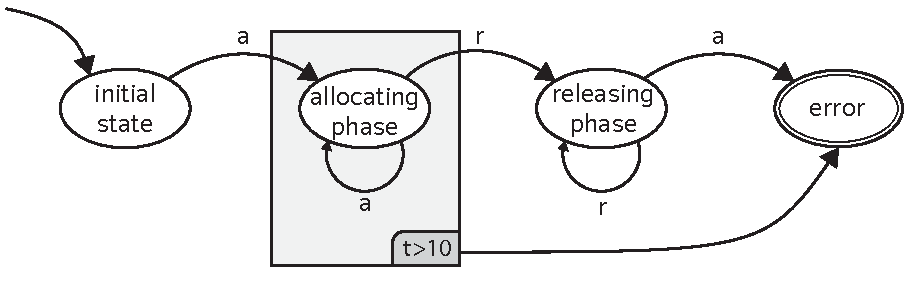
\includegraphics[width=0.7\linewidth]{figures/chapter_4/allocating_timed}
			\caption{Timed region event automaton of the two phase locking example \redraw}
			\label{fig:cep:trea}
			\end{figure}


		
	\section{Parametric Timed Regular Expression}

		Complex systems usually have parametric behaviors, which can be expressed by formalisms extended with parameters. In this section we overview such formalisms that generate the parametric timed regular languages and an automaton formalism accepting them.

		


		\begin{dfn}
		A Parametric Timed Regular Expression is a timed regular expression where the set of events are defined as a set of tuples, $\langle \Sigma, P \rangle$,
		where $\Sigma$ is defined as formerly and $P$ is a set of parameters.
		\end{dfn}
		
		


		With parametric timed regular expressions the example can be extended regular expression with parameters. \\
		$(a[i] a[i]^\ast  r[i] r[i]^\ast a[i]) | (<a[i] a[i]^\ast r[i]>_{t > 10} )$ \\
		Note that this allows us to have only one instance of the automaton even for multiple tasks, each with its own ID.
	
		\subsection{Parametric Timed Region Automaton}
			
			\todo{This subsection requires some more definition on the matter}
			
%			According to\citep{qea} we use $s$ to denote a tuple $\langle s_0,\dots,s_k \rangle$. We use $X \rightarrow Y$ and $\rightharpoondown$ to denote sets of total and partial function between
%			$X$ and $Y$, respectively. We write maps (partial functions) as $[x_0 \mapsto v_0,\dots,x_i \mapsto v_i]$ and the empty maps as $[]$. Given two maps $A$ and $B$,
%			the map override operator is defined as:
%				\[
%				 (A \dagger B)(x) = 
%				  \begin{cases} 
%				   B(x) & \text{if } x \in \text{\underline{dom}(B)} \\
%				   A(x) & \text{if } x \notin \text{\underline{dom}(B)} \text{ and } x \in \text{\underline{dom}(A)} \\
%				   \text{undefined otherwise.}
%				  \end{cases}
%				\]
%				
%			
%			\begin{dfn}
%				(Symbols, Events, Alphabets and Traces).
%				Let $\mathit{Sym} = \mathit{Val} \cup \mathit{Var}$ be the set of all symbols (variables or values).
%				An event is a pair $\langle e, \overline{s} \rangle \in \Sigma \times \mathit{Sym}^\ast,$ written $e(\overline{s})$.
%				An event $e(\overline{s})$ is ground if $\overline{s} \in \mathit{Val}^\ast$.
%				Let Event be the set of all events and GEvent be the set of all ground events.
%				A trace is a finite sequence of ground events.
%				Let Trace = $GEvent^\ast$ be the set of all traces\citep{qea}. 
%			\end{dfn}
%			
%			\begin{dfn}
%				(Substitution).
%				The binding $\theta = [x_0 \mapsto v_0, \dots, x_i \mapsto v_i]$ can be applied to a symbol $s$ and to an event
%				$e(\overline{s})$ as follows: 
%				\[
%				 s(\theta) = 
%				  \begin{cases} 
%				   \theta(s) & \text{if } s \in \underline{dom}(\theta) \\
%				   s & \text{otherwise}
%				  \end{cases}
%				  \qquad e \langle s_0,\ldots,s_j \rangle (\theta) = e \langle s_0(\theta),\ldots,s_j(\theta) \rangle
%				\]
%			\end{dfn}
%			
%			\begin{dfn}
%				(Matching).
%				Given a ground event $a$ an event $b$ the predicate matches ($a, b$) hold if there exists a binding $\theta$ s.t. $b$($\theta$) = $a$.
%				Moreover let matches($a,b$) denote the smallest such binding w.r.t $\sqsubseteq$ iff it exists (and is undefined otherwise)\citep{qea}
%			\end{dfn}
%			
%			\begin{dfn}
%				(Configurations and Transition Relation).
%				We define configurations as elements o the set Config = Q $\times$ Bind. Let $\rightarrow \subseteq$ Config $\times$ GEvent $\times$ Config be a relation on
%				configurations s.t. configurations $\langle q, \varphi \rangle$ and $\langle q', \varphi' \rangle$ are related by the ground event a, written
%				$\langle q, \varphi \rangle \xrightarrow{\text{a}} \langle q' \varphi' \rangle$ if, and only if
%					\begin{align}
%						\exists b \in \mathcal{A}, & \exists \gamma \in Assign : (q, b, \gamma, q') \in \delta \wedge \\
%						&matches(a,b) \wedge \varphi' = \gamma(\varphi \dagger match(a,b))
%					\end{align}
%				Let the transition relation $\rightarrow_{E}$ be the smallest relation containing $\rightarrow$ such that for any event
%				$a$ and configuration $c$ if $\nexists c' : c \xrightarrow{\text{a}} c'$ then $ c \xrightarrow{\text{a}}_E c$.
%				The relation $\rightarrow_E$ is lifted to traces.
%				For any two configurations $c$ and $c'$, $ c \xrightarrow{\text{$\epsilon$}}_E c$ holds, and $\xrightarrow{\text{a.$\tau$}}_E c'$ holds
%				if there exist a configuration $c'$ s.t. $c \xrightarrow{\text{a}}_E c'' \xrightarrow{\text{$\tau$}}_E c'$\citep{qea}
%			\end{dfn}
			
			
			\begin{dfn}
				\label{dfn:cep:ptrea}
				A Parametric Timed Region Event Automaton $\langle Q,\Sigma,\delta,q_0, F, t, T \rangle$ where
				\begin{itemize}
					\item $Q, \Sigma, q_0, F,$ and  $t$ are the same as in \cref{dfn:cep:trea},
					\item $T$ is a set of timeout clock variables for sets of states, for each token, i.e.~a set of tuples $\langle R, \RR, B \rangle$, where $B$ is a binding,
					\item and $\delta$ is the union of discrete and timed transitions i.e.~$\delta_t \cup \delta_d$ where
					\begin{itemize}
						\item $\delta_d$ is defined as in \cref{dfn:cep:trea},
						\item and $\delta_t$ represents timed transitions and defined as the set of tuples $\langle R \times \mathbb{R} \times Q \rangle$.
					\end{itemize}
				\end{itemize}
			\end{dfn}
			
			We give the following semantics to the parametric timed region automaton:
			
			We have to define rules for the initialization of the automaton,
			entering states with timed outgoing transitions 
			and we also define the general rules of changing states. 
			
			\begin{enumerate}
				\item Initialization Rule : On initialization of the automaton, $T$ is an empty set
				i.e.~$T = \emptyset$
			
				\item Entering new timed region rule :
				If the token enters enter a new set of timed regions, with a with binding $b$ 
				i.e.~$r^+ \neq \emptyset$, 
				we set the timers according to the timeouts, 
				i.e.~$\forall t_{timeout} : t_{timeout} \coloneqq t + t_i $ where $ r_t \in r^+, \exists q ,\delta_t\langle  r_t,t_i,q \rangle, T \langle r_t,b, t_{timeout} \rangle$
				
				\item Firing Transitions Rule: Choose an enabled transition from the set of enabled discrete or timed transitions. 
				We have two cases, the chosen transition is:
					\begin{enumerate}
						\item Discrete Transition: In case of $r^- = \emptyset$ than the execution of the transition is as in described formerly. 
							If else if we exit a region i.e.~$r^- = \emptyset$, 
							then the following rule extends the firing rule of discrete transitions:
							$\forall t_s, \forall q_s$ in $ \delta_t \langle r_i, t_s, q_s \rangle$ where $r_i \in r^-$, the timer of the regions are invalidated i.e.~
							$t_s \coloneqq \infty$
						\item Timed Transition: The transition with the minimal timeout value is selected, 
							 i.e.~transition $\exists t_i, \exists s_i, \delta_t \langle r_i, t_i, s_i \rangle$ where $ r_i \in r$ and $t_{min}$ is the minimum from all $t_i$,
							 than the following rules apply:
							 the global time is set $t \coloneqq t_{min}$, 
							 the local clock is set to infinity: $t_s \coloneqq \infty$ 
							 and move to the next state according to $\delta_t$.
					\end{enumerate}			
			\end{enumerate}

			Using the parametric timed region automaton we can compile our timed regular expression 
			$(a[i] a[i]^\ast  r[i] r[i]^\ast a[i]) | (<a[i] a[i]^\ast r[i]>_{t > 10} )$ into the automaton on \cref{fig:cep:ptrea}.


			\begin{figure}[h]
			\centering
			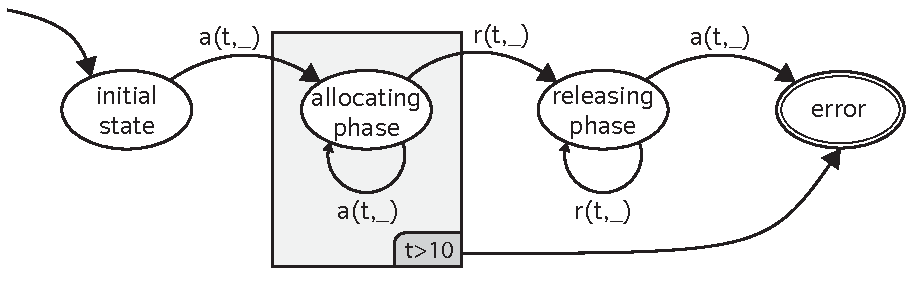
\includegraphics[width=0.7\linewidth]{figures/chapter_4/allocating_timed_parametric}
			\caption{Parametric timed region event automaton of the two phase locking example \redraw}
			\label{fig:cep:ptrea}
			\end{figure}

	\subsection{Summary of Formalisms}

	\begin{figure}[h]
	\centering
	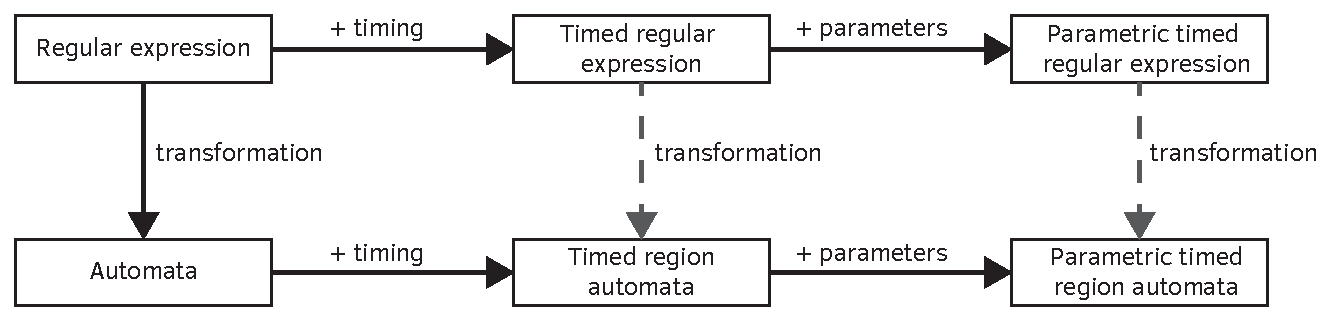
\includegraphics[width=0.95\linewidth]{figures/chapter_4/folyamatabra}
	\caption{Overview of the formalisms \redraw}
	\label{fig:cep:folyamatabra}
	\end{figure}

	The previously defined formalisms and their relations are show on \cref{fig:cep:folyamatabra}.
	The dashed arrows shows the transformations, requiring more detailed elaboration of the literature.

	\paragraph{Transformation from Regular Expression to Automaton}
	The solution is long known in the literature, see for example \citep{lam2006compilers}.

	\paragraph{Transformation from Timed Regular Expressions to Timed Automaton}
	Constructing a nondeterministic timed automaton from timed regular expressions is possible. This yields an automaton with $\epsilon$-transitions. However determinising the nondeterminstic automaton constructed from a timed regular expression is not a solved problem \emph{yet}. However, ther are some results regarding the transformation from a subset of MTL to deterministic timed automaton~\citep{nivckovic2010mtl}.

	Testing whether a timed automaton is determinizable has been proved undecidable\citep{finkel2006undecidable}.
	Also, the undecidability of universality has been further investigated, and rather restricted classes of timed automata suffer from that undecidability result. On the other hand, classes of timed automata have been exhibited, that either can be effectively determinized (for instance event-clock timed automata \citep{alur1994determinizable}, or timed automata
	with integer resets \citep{suman2008timed}), or for which universality can be decided (for instance
	single-clock timed automata \citep{ouaknine2004language}).\citep{baier2009timed}.
	This means that we need further research in this direction, to find out whether nondeterministic timed region automatons generated from timed regular expressions can be determinized, or not.

	\paragraph{Transformation from Parametric Timed Regular Expressions to Parametric Timed Automaton}
	Constructing a nondeterminsitic parametric timed region automaton from a parametric timed regular expression is possible according to the results know for timed regular expressions. As parametric automata are always nondeterminstic, thanks to the possibility of multiple tokens, we have no intention to determinize such automata.
	However, at least the $\epsilon$-transitions should be eliminated from the automata, for the purpose of efficient execution, and analysis.

	To our best knowledge, there are no results about eliminating $\epsilon$-transitions from a parametric time region automaton, being generated from parametric timed regular expression.



			
\section{Implementation}

	The currently implemented parts of the intermediate language are the following: the formal intermediate language (parametric timed regular expression), a parametric timed automaton 
	implementation, and a prototype mapping between the two.


\todo{Create a valid figure of the EMF model.}

%		\begin{figurepage}
%		  \includegraphics[width=\linewidth]{include/figures/chapter_5/model}
%		  \captionof{figure}{Metamodel of the Parametric Timed Region Automaton Impementation in EMF}
%		  \label{fig:cep:model}
%		\end{figurepage}

	\subsection{Parametric Timed Region Event Automaton}
	

	
		\subsubsection{Finite Automaton}
			The event automaton logic is represented by the State, Transition, and EventGuard classes.
			Every State has a boolean flag to show whether it is an acceptor state or not.
		\subsubsection{Timing}
			Timed regions of the formalism are represented by the Timed Region class, which consists of a set of states and the corresponding timeout value.
		\subsubsection{Parameters and Bindings}
			The parametrization of the events is represented by the Parameter abstract class. The type of each parameter is implemented with a reference to a SymbolicEvent instance. Parameters can be Fix or Free, an Event only has Fix parameters, but the tokens can have both. Event parameters can be binded to fix values or to a token parameter, this is done by the ConstantBinding and TokenParameterBinding respectively.
			
		\subsubsection{Executor}
			The algorithm first searches for all the activated transitions.
			If it finds an activated transition, it iterates over the tokens which in on that state. The first token with matching (non-confronting)
			parameter list will be split to the next state if there are new parameter bindings from the event, or moved if there are no new bindings.
			If a token enters an acceptor state it will trigger a function call.

	\subsection{Parametric Timed Regular Expression}

		Currenly the regular expression has a grammar implemented in Xtext, which generates a textual editor, and can parse 
		textual input to an EMF model. This EMF model can be transformed later. 
		
		The grammar is the following:

		\lstinputlisting[language=Xtext]{ptregex.xtext}

		Note that the parameter listing is inside with square brackets ``[]'' to make the language context free. If we would use the simple round brackets, then A(B) would be ambiguous -- it could be either an A event with a B parameter, or a simple sequence of event A and event B with an unnecesary bracket.

	\subsection{Transformation from Regular Expression to Automaton}

		The transformation of simple (not timed and parametric) regular expressions are well known in the current literature. The various algorithms were investigated and a chosen algorithm from \citep{lam2006compilers}  is implemented.
		Extensions by timing and parameters are considered future work.

		\subsubsection{Regular Expression to Nondeterministic Automaton with $\epsilon$ transitions}
			First the regular expression is transformed to a nondeterministic automaton with the following rules:

			\begin{figure}[h]
			\centering
			\includegraphics[width=0.3\linewidth]{figures/chapter_4/subexpression_event}
			\caption{Constructed NFA from the simple event $a$ \redraw}
			\label{fig:cep:nfaevent}
			\end{figure}

			\begin{figure}[h]
			\centering
			\includegraphics[width=0.5\linewidth]{figures/chapter_4/subexpression_sequence}
			\caption{Constructed NFA from the sequence $N(s)N(t)$ \redraw}
			\label{fig:cep:nfasequence}
			\end{figure}

			\begin{figure}[h]
			\centering
			\includegraphics[width=0.5\linewidth]{figures/chapter_4/subexpression_choice}
			\caption{Constructed NFA from the choice $N(s)|N(t)$ \redraw}
			\label{fig:cep:nfachoice}
			\end{figure}

			\begin{figure}[h]
			\centering
			\includegraphics[width=0.5\linewidth]{figures/chapter_4/subexpression_asterisk}
			\caption{Constructed NFA from the closure $N(s)^*$ \redraw}
			\label{fig:cep:nfasterisk}
			\end{figure}

		\needspace{5cm}
		\subsubsection{Determinizing the automaton}

			The algorithm is introduced on \cref{alg:cep:subset}.
			The algorithm constructs a transition table $\mathit{Dtran}$ for $D$. Each state of $D$ is a set of NFA states, and we construct $\mathit{Dtran}$ so $D$ will simulate ``in paralell'' all possible moves $N$ can make on a given input trace. Our first problem is to deal with $\epsilon$-transitions of $N$ properly.


			Move($T,a$) is the set of states of the NFA which there is a transition on input symbol $a$ from some state in $T$.

			\begin{algorithm}
			\SetAlgoLined
			\SetKwInOut{Input}{input}\SetKwInOut{Output}{output}
			\Input{An NFA $N$}
			\Output{A DFA $D$ accepting the same language as $N$}
			initially, $\epsilon$-closure($s_0$) is the only state in $\mathit{Dstates}$, and it is unmarked\;
			\While{there is an unmarked state $T$ in $\mathit{Dstates}$}{
				mark $T$\;
				\ForEach{input symbol $a$}{
					$U = $ $\epsilon$-closure(move($T,a$))\;
					\If{$U$ is not in $\mathit{Dstates}$}{
						Add $U$ as an unmarked state to $\mathit{Dstates}$\;
					}
					$\mathit{Dtran}[T,a] = U$ \;
				}
			}
			\caption{The subset construction of a DFA from an NFA}
			\label{alg:cep:subset}
			\end{algorithm}



			\begin{algorithm}
			\SetAlgoLined
			\SetKwInOut{Input}{input}\SetKwInOut{Output}{output}
			\Input{A set of states $T$}
			\Output{A set of states $\epsilon$-closure($T$)}
			push all states of $T$ onto $\mathit{stack}$\;
			initialize $\epsilon$-closure($T$) to $T$\;
			\While{$\mathit{stack}$ is not empty}{
				pop $t$ from the $\mathit{stack}$ \;
				\ForEach{state $u$ with an edge from $t$ to $u$ labeled $\epsilon$}{
					\If{$u$ is not in $\epsilon$-closure($T$)}{
						Add $u$ to $\epsilon$-closure($T$)\;
						push $u$ onto $\mathit{stack}$ \;
					}
				}
			}
			\caption{Computing $\epsilon$-closure($T$)}
			\end{algorithm}

	\subsection{VEPL to Regular expressions}
		Regular expressions can be built from VEPL patterns, taking the event contexts into consedaration.
		Strict immediate is show on \cref{tab:cep:vepl_regex_strict}, and Chronicle is shown on \cref{tab:cep:vepl_regex_chronicle}.
		Each of the patterns must start with a $\Sigma^*$, as in Complex Event Processing every pattern might have arbitrary prefix.


		\begin{table}
		\caption{Basic VEPL operators in strict immediate context, expressed with regular expressions}		
		\label{tab:cep:vepl_regex_strict}
			\begin{tabularx}{0.5\textwidth}{llX}
				\toprule
				VEPL operator &	Regular Expression \\
				\midrule
				$p_1$ $\rightarrow$ $p_2$ & $p_1$ $p_2$ \\
				$p_1$ OR $p_2$ & $p_1|p_2$ \\
				$p\{\ast\}$ & $p^*$ \\
				$p[t]$ & $p[t]$ \\ 
				\bottomrule
			\end{tabularx}
		\end{table}

		\begin{table}
		\caption{Basic VEPL operators in chronicle context, expressed with regular expressions}		
		\label{tab:cep:vepl_regex_chronicle}
			\begin{tabularx}{0.5\textwidth}{llX}
				\toprule
				VEPL operator &	Regular Expression \\
				\midrule
				$p_1$ $\rightarrow$ $p_2$ & $p_1$ $(\Sigma/(p_2))^*$ $p_2$ \\
				$p_1$ OR $p_2$ & $p_1|p_2$ \\
				$p\{\ast\}$ & nothing\\
				$p[t]$ & $p[t]$ \\
				\bottomrule
			\end{tabularx}
		\end{table}
	
	